\documentclass[12pt]{article}
\usepackage{amsmath}
\usepackage{amssymb} %mathbb
\usepackage{graphicx}
\usepackage{hyperref}
\usepackage{xcolor}
\usepackage{cancel}
\usepackage[latin1]{inputenc}
\usepackage[paperheight=377mm,paperwidth=210mm,top=1.0cm,bottom=1.3cm,left=1.0cm,right=1.0cm,landscape]{geometry}

\begin{document}

\Large

\begin{center}
\textbf{Teoria Geom\'etrica da Medida | Capacidade}
\end{center}

\large

V\'ideo Principal no \href{https://www.youtube.com/watch?v=mmzqmIcX7xo}{\color{blue}\underline{YouTube}}.

\vspace{3mm}

		\begin{center}
		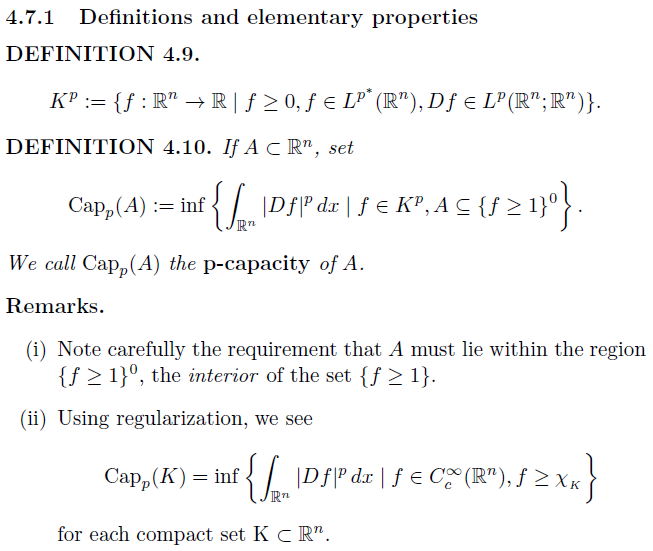
\includegraphics[scale=.9]{1}
		\end{center}

4.9 Lebesgue $p \le \infty$ integr\'aveis.

4.10 Interior de $\{ x\,;\,f(x) \ge 1 \}$.

(ii) Troque $A$ por compacto $K$. fun\c{c}\~oes de suporte compacto tais que $f(x) \ge 1, \forall x \in K$ e $f(x) \ge 0, \forall x \notin K$.

\vspace{300mm}

		\begin{center}
		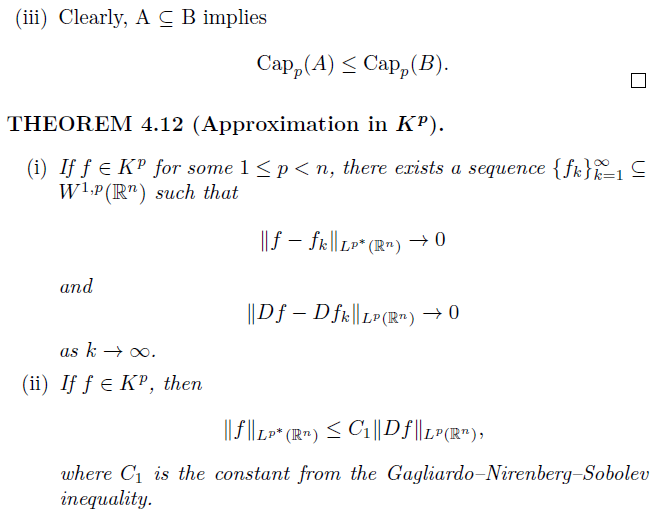
\includegraphics{2}
		\end{center}

(iii) Trocando $A$ por $B$, o \'infimo aumenta.

(i) $f_k$ tende a $f$ em norma. A derivada de $f_k$ tende \'a derivada de $f$ em norma.

(ii) $\bigg\Vert \cfrac{f'}{f} \bigg\Vert \ge C_1 \Rightarrow \ln f(t) \ge C_1 t \Rightarrow f(t) \ge e^{C_1 t}$.

\vspace{300mm}

		\begin{center}
		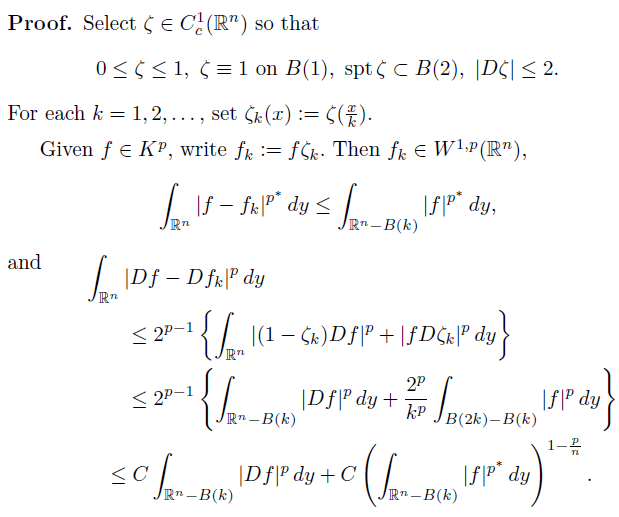
\includegraphics[scale=.9]{3}
		\end{center}

Gr\'afico de zeta em fun\c{c}\~ao do raio. zeta \'e $1$ dentro, $0$ fora e m\'odulo da derivada de zeta menor ou igual a $2$ no meio. $\zeta(x), \zeta\bigg(\cfrac{x}{2}\bigg), \zeta\bigg(\cfrac{x}{3}\bigg), \cdots \to \zeta(0)$.

$f_k \in $ espa\c{c}o de Sobolev, subespa\c{c}o de $L^p$ onde $I(u) = \int_\Omega \vert \nabla u \vert^2\,\mathrm{d}x$ est\'a bem definido.

$\int_R f = \int_{R - B} f + \int_B f$. Tende a zero, pela regi\~ao de integra\c{c}\~ao.  $2\cdot |a + b|^p \le |2a + 2b|^p \le |2a|^p + |2b|^p \therefore |a + b|^p \le \cfrac{|2a|^p + |2b|^p}{2}$.

$Df - \zeta_k Df + \zeta_k Df - Df(\zeta_k) = (1 - \zeta_k) Df + \underbrace{\zeta_k Df - \cfrac{Df}{d\zeta_k} \cdot \cfrac{D\zeta_k}{dx}}_{\le fD\zeta_k} \Leftrightarrow  - \cfrac{1}{f^2} \cdot \cfrac{Df}{d\zeta_k} \cdot \cfrac{D\zeta_k}{dx} \le \cfrac{f D\zeta_k - \zeta_k Df}{f^2} \Leftrightarrow D\bigg( \cfrac{1}{f(\zeta_k)} \bigg) \le D\bigg( \cfrac{\zeta_k}{f} \bigg)$.

$D\zeta_k \le \cfrac{1}{k}\cdot 2 = \cfrac{2}{k}$. Regra da cadeia. Trocamos o expoente, por causa de Gagliardo Nirenberg Sobolev, na p\'agina $138$ do livro-texto. Tende a zero.

\vspace{300mm}

		\begin{center}
		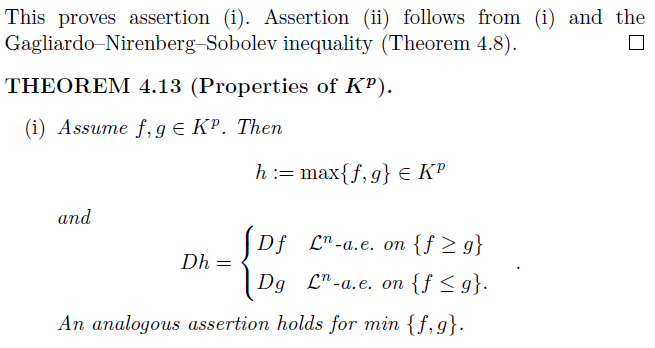
\includegraphics{4}
		\end{center}

$f_k \to f.\,Df_k \to Df.$ Integral de p*-norma $\le C_1\cdot$ Integral de p-norma. Ent\~ao $\Vert f\Vert \le C_1\cdot \Vert Df\Vert$.

\vspace{3mm}

O max e o min est\~ao em $K^p$.

Diferencial do m\'aximo igual a diferencial de $f$ q.t.p. para todo x onde $f(x) \ge g(x)$.

Analogamente, diferencial do m\'inimo igual a diferencial de $g$ q.t.p. para todo x onde $f(x) \ge g(x)$.

\vspace{3mm}

Diferencial do m\'aximo igual a diferencial de $g$ q.t.p. para todo x onde $f(x) \le g(x)$.

Analogamente, diferencial do m\'inimo igual a diferencial de $f$ q.t.p. para todo x onde $f(x) \le g(x)$.

\vspace{300mm}

		\begin{center}
		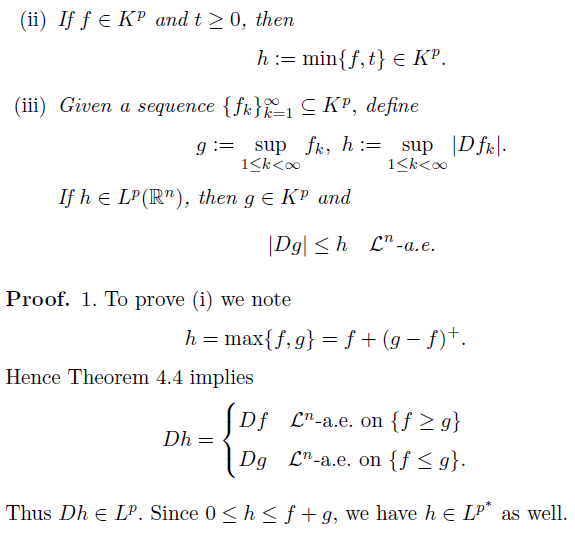
\includegraphics{5}
		\end{center}

$h$ est\'a em $K^p$.

O supremo das $Df_k$ est\'a em $L^p$. O supremo das $f_k$ est\'a em $K^p$. A derivada deste \'ultimo em m\'odulo \'e sempre $\le$ o outro q.t.p.

Prova

Teorema 4.4: Parte positiva e parte negativa. $Df^+ = Df.\,\,Df^- = - Df$.

A diferencial est\'a em $L^p$. $h$ \'e limitada.

\vspace{300mm}

		\begin{center}
		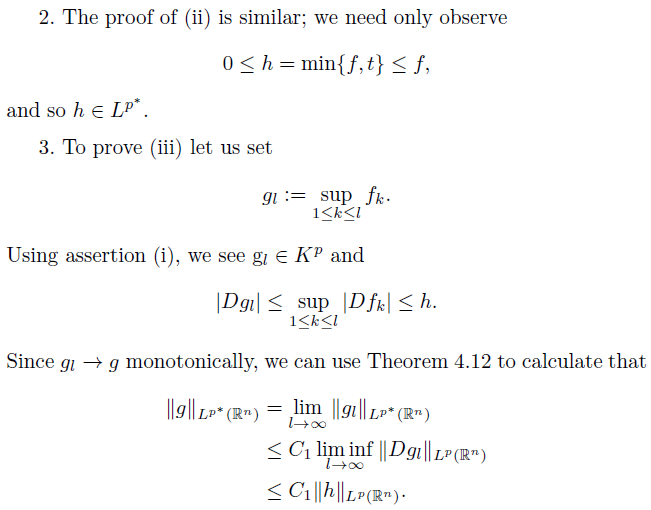
\includegraphics{6}
		\end{center}

Teorema 4.4: Parte positiva e parte negativa. $Df^+ = Df.\,\,Df^- = - Df$.

A diferencial est\'a em $L^p$. $h$ \'e limitada.

\vspace{3mm}

(3) $\Vert g \Vert \le C_1 \Vert h \Vert$.

\vspace{3mm}

Queremos agora mostrar que $\overline{L}(\phi) = \int_{\mathbb{R}^n} \langle \phi, k\rangle \,\mathrm{d}y$ com $\vert k \vert < h$ q.t.p. onde $L(\phi) = \int_{\mathbb{R}^n} g \langle \nabla, \phi \rangle\,\mathrm{d}y$.

Vai seguir pelo teorema da representa\c{c}\~ao de Riesz que $g \in K^p$ e portanto $\vert Dg\vert \le h$ q.t.p.

\vspace{300mm}

		\begin{center}
		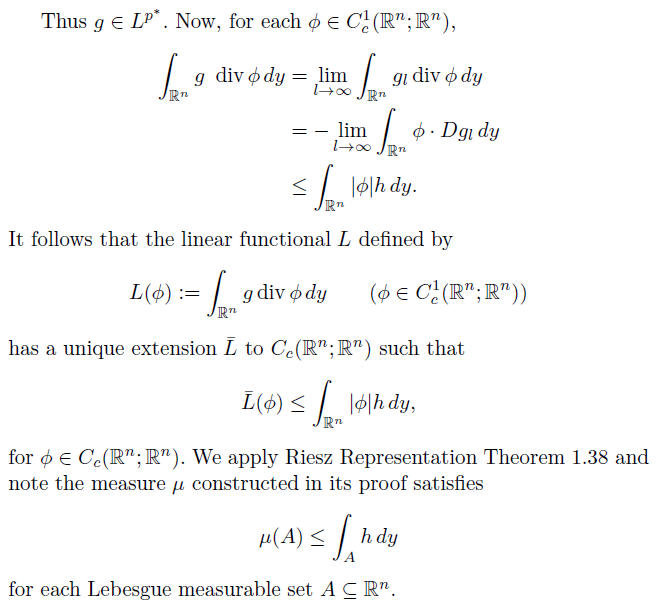
\includegraphics[scale=.9]{7}
		\end{center}

$g_\ell \cdot \cfrac{\partial \varphi}{\partial x} + \varphi \cdot \cfrac{\partial g_\ell}{\partial x} = 0$. Regra do produto. $D \langle g_\ell \cdot \varphi \rangle = 0 \Leftrightarrow \langle g_\ell, \varphi\rangle = $ constante.

Por defini\c{c}\~ao, $h = \sup \vert Df_k \vert$.

Extens\~ao de classe $C^1$ para classe $C^0$. A extens\~ao \'e menor ou igual \`a integral de $\vert \phi\vert h$.

No meio da prova de Riesz, a medida constru\'ida satisfaz a \'ultima desigualdade para todo conjunto Lebesgue-mensur\'avel $A$ em $\mathbb{R}^n$.

\vspace{300mm}

		\begin{center}
		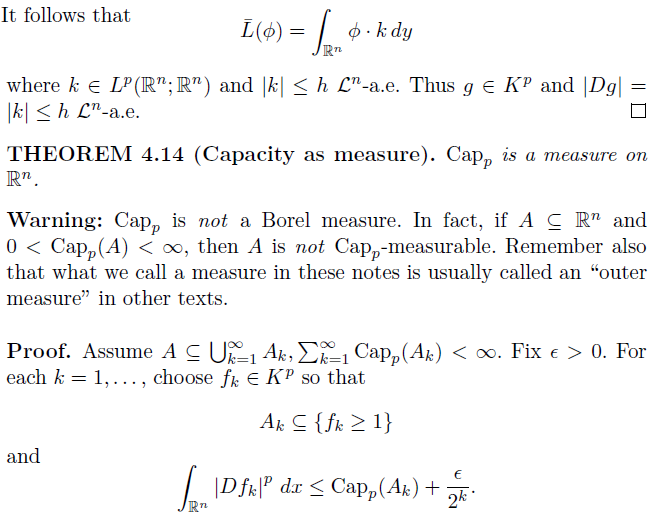
\includegraphics{8}
		\end{center}

Extens\~ao de classe $C^1$ para classe $C^0$. A extens\~ao \'e igual \`a integral de $\langle \phi, k \rangle$. Se voc\^e preferir, \'e teorema do valor m\'edio.

Sen\~ao, \'e Cauchy-Schwarz, mesmo.

\vspace{3mm}

A medida \'e n\~ao boreliana. \'E uma medida exterior em outros autores.

\vspace{3mm}

Vamos mostrar que a capacidade de $A$ \'e exatamente o mesmo que a soma das capacidades de qualquer cobertura de $A$.

Suponha que a soma das capacidades \'e finita. Escolha $f_1, f_2, \cdots$ tais que h\'a a cota superior acima para a $L^p$-integral da diferencial.

Essa escolha \'e poss\'ivel, pois no caso mais degenerado, todas as $f_k$'s s\~ao constantes, logo t\^em derivada nula.

\vspace{300mm}

		\begin{center}
		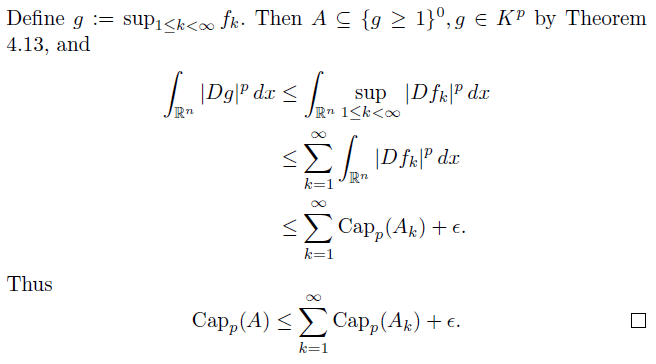
\includegraphics{9}
		\end{center}

Defina o supremo. Aplique o Teorema 4.13 e a integral \'e menor ou igual a $h$.

O supremo \`a direita \'e menor ou igual \`a soma enumer\'avel.

\'epsilon \'e arbitr\'ario. Tende a zero.

\vspace{300mm}

		\begin{center}
		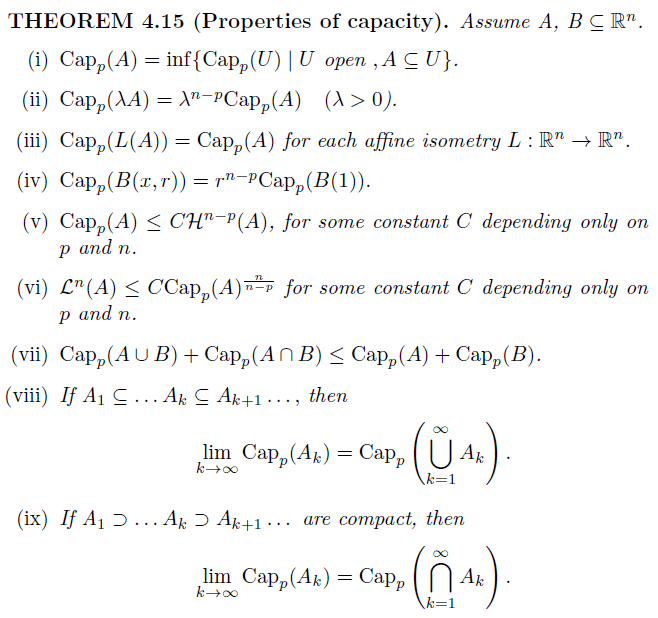
\includegraphics[scale=.9]{10}
		\end{center}

1. \'Infimo dentre todos os abertos que cont\^em $A$. 2. A constante vai para fora. 3. Invari\^ancia por isometria que preserva a origem.

4. Bola de raio $r$: capacidade diretamente proporcional a $r^{n - p}$. 5. Raz\~ao com medida de Hausdorff limitada por $C(n,p)$. 6. Medida de Lebesgue elevada a $n-p$, dividida por capacidade elevada a $n$, raz\~ao limitada por $C(n, p)$. 7. Capacidade da uni\~ao menor ou igual que soma das capacidades menos capacidade da interse\c{c}\~ao.

8. Sequ\^encia ascendente de conjuntos. capacidade do limite igual a capacidade da reuni\~ao de todos.

9. Sequ\^encia descendente de conjuntos, todos compactos. Capacidade do limite igual a capacidade da interse\c{c}\~ao de todos.

\vspace{300mm}

		\begin{center}
		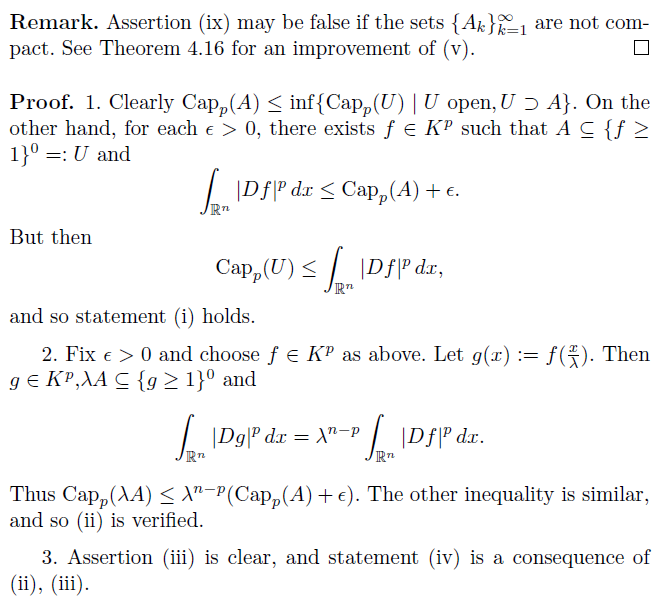
\includegraphics[scale=.85]{11}
		\end{center}

A hip\'otese de ser compacto \'e necess\'aria em 9.

1. Aumentar $A$ aumenta capacidade. Agora a volta. $C(A)$ \'e o \'infimo dos $Dfp$'s. Some $\epsilon$ ao \'infimo, existe integral. $C(U) \le \text{ integral }\le C(A) + \epsilon$.

2. Queremos mostrar que $C(B) \le k C(A) + \epsilon$. $y = \lambda a \Rightarrow g(y) = f(y/\lambda) = f(a) \ge 1$. Agora $\cfrac{Dg}{dx} = \cfrac{1}{\lambda}\cdot\text{ Id}_{n\times n} \circ \cfrac{Df}{dx}$.

Agora mostre o contr\'ario, que $k C(A) - \epsilon \le C(B) \therefore \lambda^{n - p} [\text{Cap}_p(A) - \epsilon] \le \text{ Cap}_p(\lambda A)$.

3. \'Obvio. Compare $a\in A \Rightarrow f(a) \ge 1$ com $y = Ma + a_0 \Rightarrow f(y) \ge 1$. \'Infimos sobre $a,y$.

4. Consequ\^encia de $(2)\wedge (3)$. Pegue a bola unit\'aria. $\lambda = r$ vai para fora. Transla\c{c}\~ao \'e isometria afim.

\vspace{300mm}

		\begin{center}
		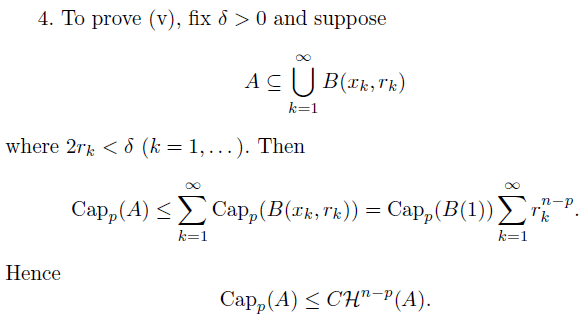
\includegraphics{12}
		\end{center}

5. Usa propriedade 4.

\vspace{300mm}

		\begin{center}
		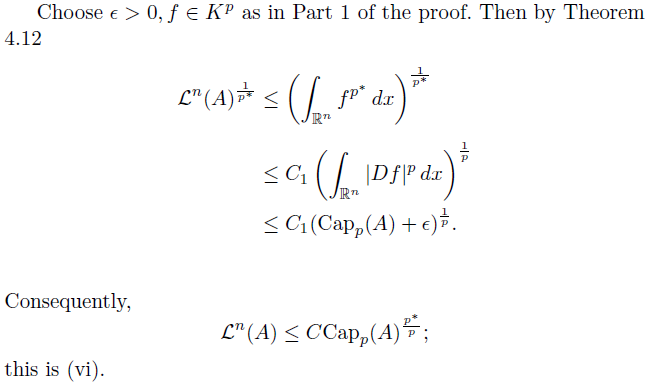
\includegraphics{12b}
		\end{center}

1. $C(A)$ \'e o \'infimo dos $Dfp$'s. Some $\epsilon$ ao \'infimo, existe integral. $C(U) \le \text{ integral }\le C(A) + \epsilon$.

6. A medida em $A$ \'e menos que a medida no espa\c{c}o todo. Aplique o teorema.

Eleve a $p^* = \cfrac{np}{n - p}$ dos dois lados.

\vspace{300mm}

		\begin{center}
		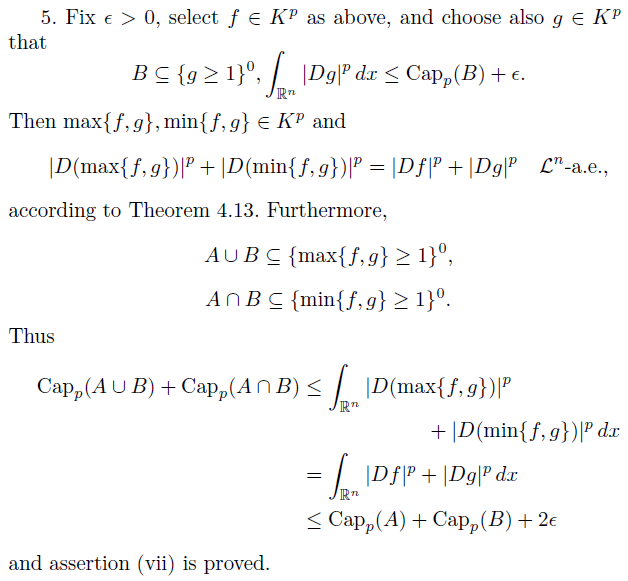
\includegraphics[scale=.9]{13}
		\end{center}

1. $C(A)$ \'e o \'infimo dos $Dfp$'s. Some $\epsilon$ ao \'infimo, existe integral. $C(U) \le \text{ integral }\le C(A) + \epsilon$.

1. $C(B)$ \'e o \'infimo dos $Dgp$'s. Some $\epsilon$ ao \'infimo, existe integral. $C(V) \le \text{ integral }\le C(B) + \epsilon$.

7. $x \in A \cup B \Rightarrow f(x) \ge 1 \vee g(x) \ge 1 \Rightarrow M = \max \ge 1$.

$x \in A \cap B \Rightarrow f(x) \ge 1 \wedge g(x) \ge 1 \Rightarrow m = \min \ge 1$.

\'Infimo \'e menos. Igual \'a linha de cima. Some $C(A) + \epsilon + C(B) + \epsilon$.

\vspace{300mm}

		\begin{center}
		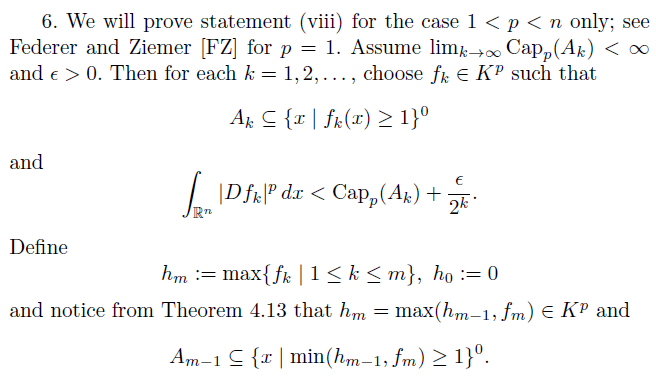
\includegraphics{14}
		\end{center}

8.1. Mais na frente, o autor usa que se a cobertura de $A$ tem capacidade finita, por 8, $A$ \'e compacto.

\vspace{300mm}

		\begin{center}
		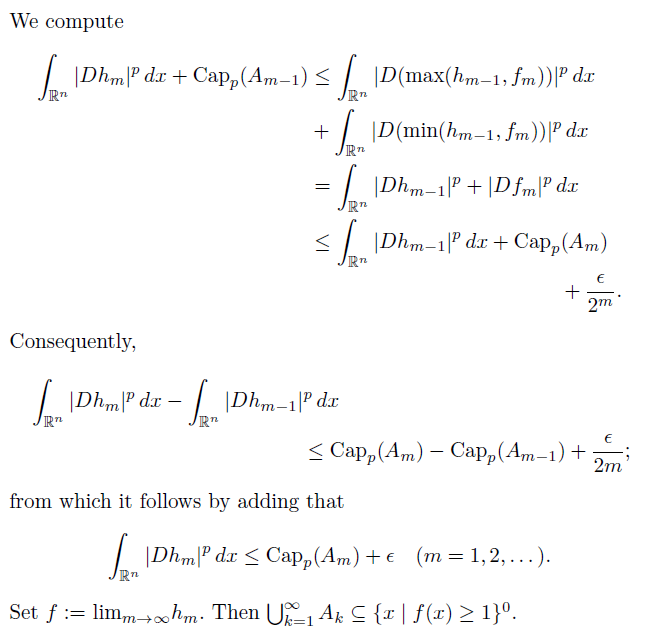
\includegraphics[scale=.9]{15}
		\end{center}

8.2. $C(A_m) + \epsilon + \int |Dh_{m-1}|^p + \cfrac{\epsilon}{2m} - \epsilon - C(A_{m - 1} \le C(A_m) + \epsilon$.

$\int |Dh_{m-1}|^p + \cfrac{\epsilon}{2m} \le C(A_{m - 1}) + \epsilon$.

\vspace{300mm}

		\begin{center}
		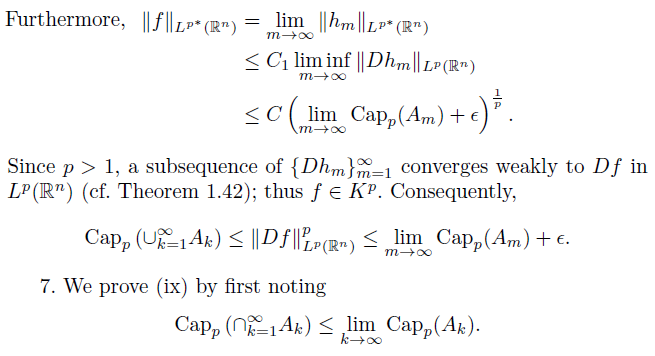
\includegraphics{16}
		\end{center}

8.3. Capacidade da reuni\~ao \'e \'infimo. Menos que $Df$. Menos que a linha de cima.

Usa teorema $3$ no livro texto p. $57$. Falta $p = 1$.

9.1. Capacidade de interse\c{c}\~ao. Menos que capacidade de um apenas. Menos que $C(U)$. \'Infimo dos $2$ lados.

\vspace{300mm}

		\begin{center}
		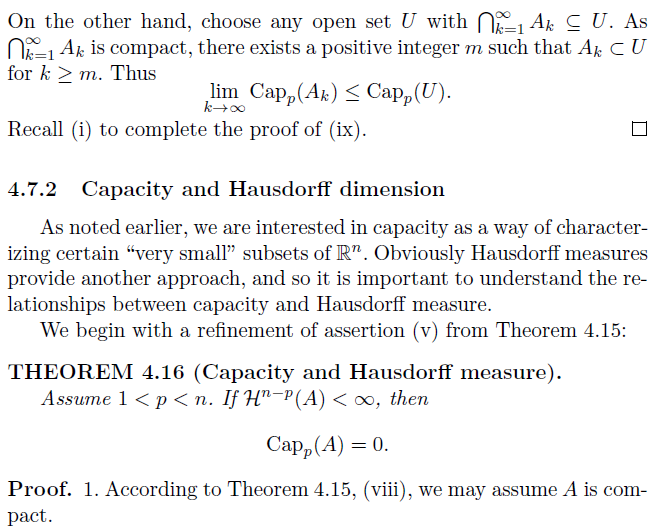
\includegraphics[scale=.9]{17}
		\end{center}

9.2. Capacidade de interse\c{c}\~ao. Menos que capacidade de um apenas. Menos que $C(U)$. \'Infimo dos $2$ lados.

16.1. Se a medida $n - p > 0$ de Hausdorff do conjunto $A$ \'e finita, ent\~ao a $p > 1$ capacidade de $A$ \'e nula.

Como j\'a dissemos, suponha sem perda de generalidade que $A$ \'e compacto.

\vspace{300mm}

		\begin{center}
		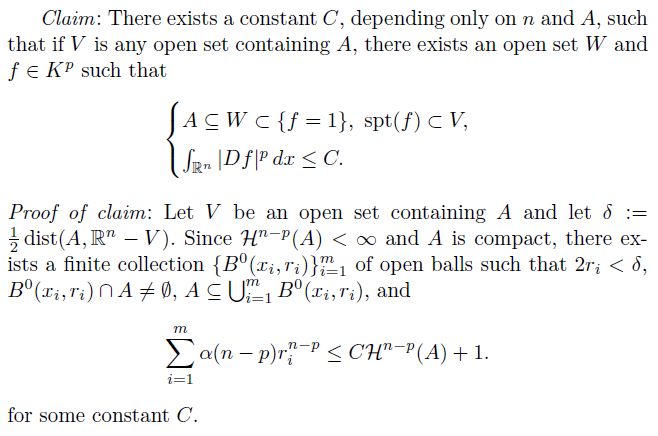
\includegraphics{18}
		\end{center}

16.2. Soma $\delta = 1$.

\vspace{300mm}

		\begin{center}
		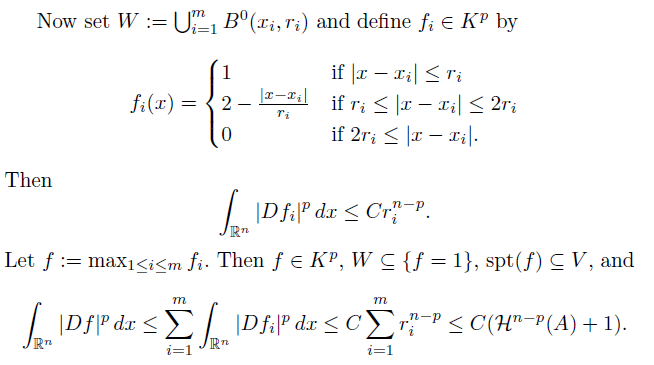
\includegraphics{19}
		\end{center}

16.3. Usa 4.15.5: $C(A) \le C\cdot H^{n-p}(A)$, depende de $n, p$.

M\'aximo. Menos que soma. Troca $\alpha$ por $1$.

\vspace{300mm}

		\begin{center}
		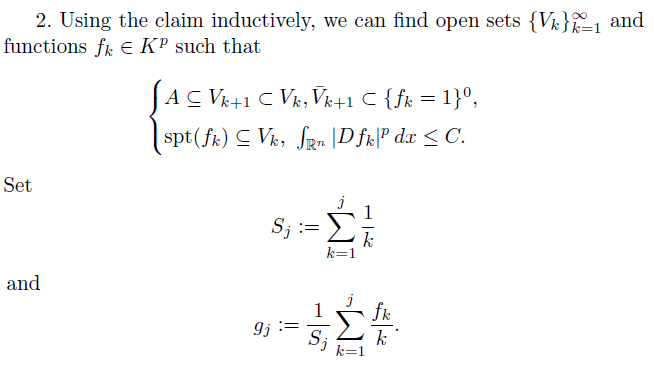
\includegraphics{19b}
		\end{center}

16.4. Indu\c{c}\~ao. Cada vez mais perto de $A$.

\vspace{300mm}

		\begin{center}
		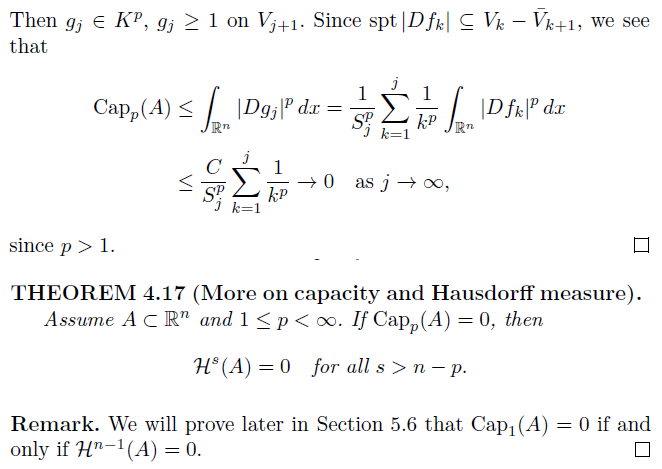
\includegraphics{20}
		\end{center}

16.5. Integral. menos que $C$.

17.1. Se a $p$ capacidade do conjunto $A \subset \mathbb{R}^n$ \'e nula, ent\~ao a medida $s > n - p$ de Hausdorff de $A$ \'e nula.

5.6. A $1$ capacidade do conjunto $A \subset \mathbb{R}^n$ \'e nula, se e somente se, a medida $s = n - 1$ de Hausdorff de $A$ \'e nula.

\vspace{300mm}

		\begin{center}
		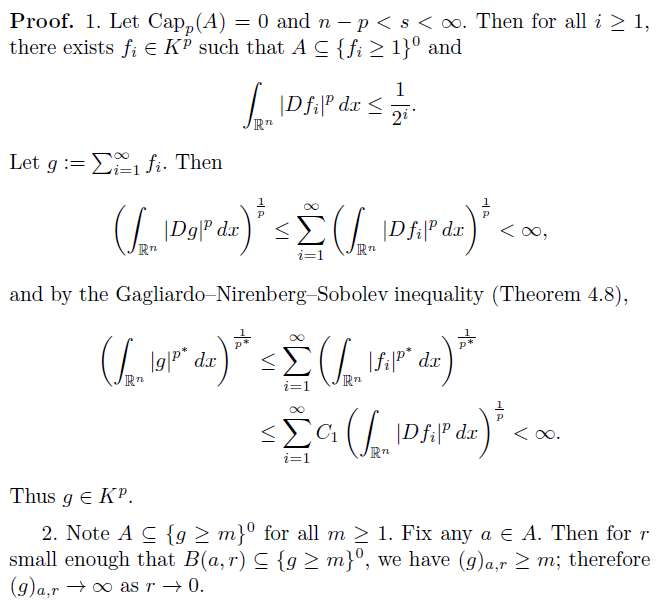
\includegraphics[scale=.9]{21}
		\end{center}

17.2. Passo $1$. Queremos mostrar que $g \in K^p$.

$1/2, 1/3, 1/4, \cdots \to 0$.

Progress\~ao geom\'etrica.

Passo $2$. $g$ tem cota m\'inima. Cada vez maior.

\vspace{300mm}

		\begin{center}
		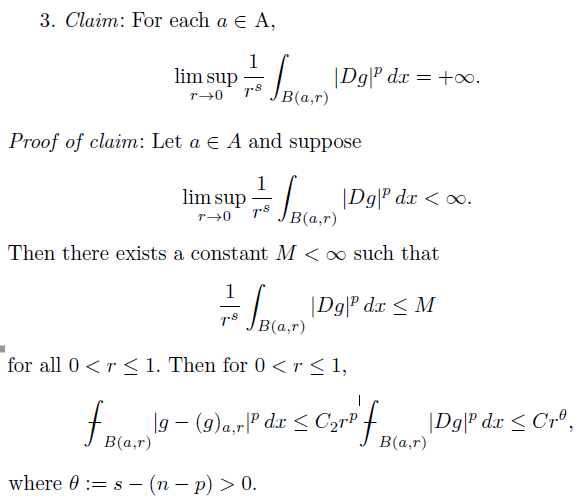
\includegraphics{22}
		\end{center}

17.3. $|g - m| \le C_2^{1/p}\cdot r \cdot |Dg|$. Troca $p \le p + s - n$.

Pr\'oximo passo, vamos integrar $g - m$.

\vspace{300mm}

		\begin{center}
		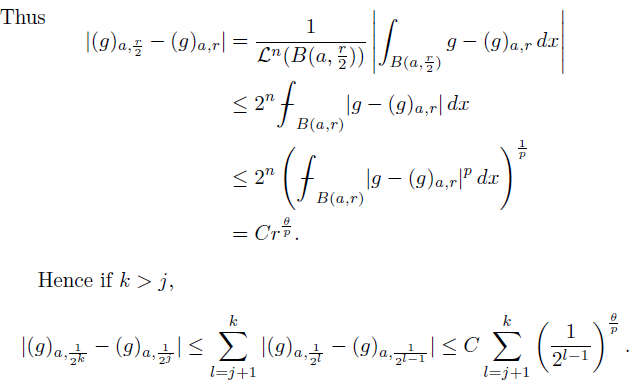
\includegraphics{23}
		\end{center}

17.4. Dobrou o raio. Norma $1$, menos que norma $p$.

Embutiu $2^n$ em $C$.

$r := \cfrac{1}{2^{\ell-1}}$.

\vspace{300mm}

		\begin{center}
		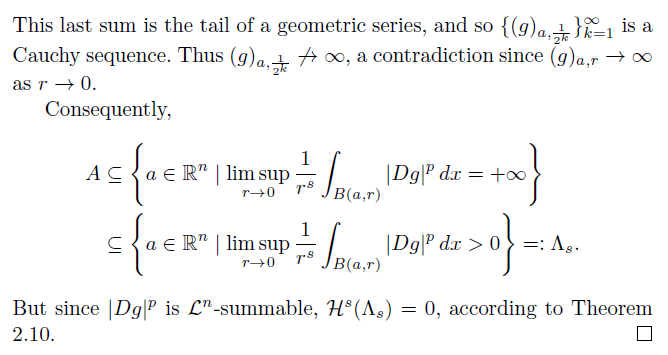
\includegraphics{24}
		\end{center}

17.5. Absurdo.

2.10. livro-texto p. $77$.

\vspace{12mm}

\Large

\begin{center}
\textbf{Obrigado}
\end{center}

\large

\vspace{12mm}

Fora da caridade, n\~ao h\'a salva\c{c}\~ao. Com caridade, h\'a evolu\c{c}\~ao.

Vinicius Claudino Ferraz, vers\~ao $0.2$ de 11/fev/2020.

\end{document}
